\documentclass[11pt, a4paper]{article}
\usepackage{microtype}
\usepackage{amsmath}
\usepackage{mathtools}
\usepackage{amssymb}
\usepackage{booktabs}
\usepackage{array}
\usepackage[margin=1in]{geometry} % set page margins automatically
\usepackage{siunitx}
\usepackage{graphicx}
\usepackage{lmodern}  % better i18n Postscript version of Knuth's cm fonts
\usepackage{url}
\usepackage[parfill]{parskip}
\usepackage[T1]{fontenc}
\usepackage[italian]{babel}
\usepackage{mhchem}
\usepackage{fancyvrb}
\usepackage{hyperref}
\usepackage{graphicx}
\usepackage{float}
\usepackage[bottom]{footmisc}
\usepackage{siunitx}
\usepackage{textgreek}
\usepackage{subcaption}

\listfiles

\DeclareSIUnit{\sample}{S}
\DeclareSIUnit{\atm}{atm}
\DeclareSIUnit{\molar}{M}

\begin{document}

\title{\vspace{-6em}\huge{Relazione di laboratiorio 4}\vspace{-2ex}}
\author{Gianluca Zappavigna}
\maketitle

\section{Introduzione}

% \begin{figure}[H]
    %     \centering
    %     \includegraphics[width=0.4\textwidth]{pic.jpg}
    % \end{figure}

Lo scopo di questa esperienza è studiare la cinetica di rilegame tra il monossido di carbonio (\ce{CO}) e la mioglobina (\ce{Mb})
a seguito della dissociazione provocata da un impulso laser della durata di pochi nanosecondi (nanosecond flash photolysis).

Questa tecnica sfrutta il fatto che il legame \ce{Fe-CO} nell'eme delle globine è fotolabile, ed è possibile ottenere un'efficienza di fotolisi del 100\%.
È importate che il flash laser duri pochi \unit{\nano\second} perché ci interessa studiare la cinetica di rilegame anche a tempi molto brevi.

Infatti la cinetica della mioglobina è particolarmente complessa, in quanto è la somma di processi separati che avvengono su scale temporali diverse.
Alcune di queste scale di tempi possono essere inferiori al \unit{\micro\second}.

% (Per questa ragione la cinetica è detta multiesponenziale.)

\subsection{\texorpdfstring{\ce{CO}}{CO} vs \texorpdfstring{\ce{O_2}}{O2}}

Nelle regolari funzioni biologiche la mioglobina lega l'ossigeno molecolare \ce{O_2}.
Per questo esperimento si è scelto il \ce{CO} perché, nel caso dell'\ce{O_2}, la luce che incide sul campione può portare alla foto-ossidazione dell'eme,
cioè all'ossidazione del ferro che passa dallo stato ferroso allo stato ferrico, e contemporaneamente alla formazione di uno ione superossido \ce{O_2^-}.
La mioglobina in cui l'atomo di \ce{Fe} dell'eme ha stato di ossidazione \ce{Fe^{3+}} è detta metmioglobina (MetMb) ed è incapace di legare il substrato.
Questo effetto porterebbe ad una degradazione del campione e quindi ad una perdita di intensità del segnale. Inoltre lo ione superossido fa parte delle specie reattive dell'ossigeno (ROS) e può reagire
con le altre proteine danneggiando ulteriormente il campione.

\section{Descizione dell'esperimento}

Il rilegame viene osservato illuminando il campione con una lampada allo Xenon e misurando le variazioni di assorbanza nel tempo a seguito dell'impulso laser.

Mentre nelle esperienze precedenti effettuavamo misure di assorbanza in funzione della frequenza d'onda e in uno stato di equilibrio del campione,
in questo caso la misura viene effettuata ad una singola lunghezza d'onda in una condizione di non equilibrio.

\subsection{Apparato sperimentale}

\begin{figure}[H]
    \centering
    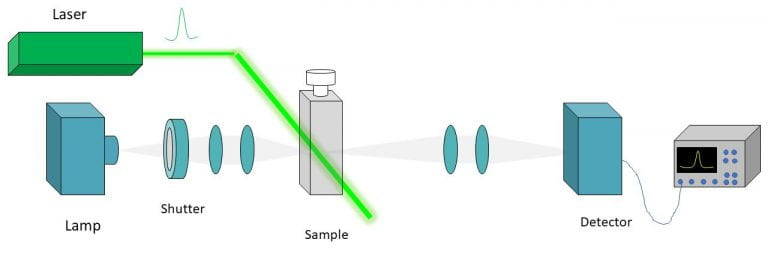
\includegraphics[width=0.7\textwidth]{FlashPhotolysis.jpg}
    \caption{Diagramma approssimativo del setup}
\end{figure}

La prima parte del setup sperimentale è composta da un laser Nd:YAg a impulsi. Il flash prodotto dal laser viene ridiretto verso il campione da un'apparato ottico.

Non viene utilizzato il fascio diretto prodotto dal laser, che ha una lunghezza d'onda di 1064 nm, ma si usa un generatore di armoniche per generare la seconda armonica, a 532 nm.
Siccome il fascio è polarizzato linearmente, per evitare effetti dovuti all'anisotropia del campione si inserisce anche una lamina quarto d'onda, così che la luce che incide
sul campione abbia polarizzazione circolare. La luce laser in uscita dal campione colpisce poi una superficie assorbente che limita gli effetti di scattering.

Perpendicolarmente al fascio laser si illumina il campione con la luce emessa da una lampada allo Xenon. Questa volta non si tratta di un impulso luminoso
ma di luce continua.
Anche in questo caso la luce non arriva direttamente al campione, ma passa attraverso un monocromatore che
seleziona solo la lunghezza d'onda a 436 nm. La ragione di questa scelta sarà motivata in seguito.

La luce della lampada che esce dal campione passa per un secondo monocromatore, che seleziona sempre la componente dello spettro alla stessa lunghezza d'onda.
Lo scopo di questo secondo monocromatore è di escludere sia la luce proveniente dal laser che per scattering arriva al detector, sia l'eventuale emissione di fluorescenza del campione.
Infine la luce trasmessa arriva al detector. Il detector è composto da un fotomoltiplicatore che traduce il debole segnale luminoso in un segnale di tensione.
Il segnale di tensione viene misurato attraverso un oscilloscopio digitale.
La luce della lampada Xe, per passare da un'elemento del setup a quello successivo (lampada, monocromatori, campione), viene collimata da una prima lente e poi focalizzata da una seconda.

Il campione viene mantenuto a temperatura costante da una cella peltier. \'E importante non avere variazioni di temperatura durante l'esperimento perché essa influenza la reattività
tra la mioglobina e il CO libero in soluzione e quindi modifica la cinetica che vogliamo misurare. Lasciare esposto il campione alla luce proveniente dalla lampada Xe renderebbe vana
la funzione della cella. Si adopera quindi uno shutter che normalmente blocca il fascio. Lo shutter viene aperto poco prima che arrivi l'impulso laser e rimane aperto solo per il tempo necessario
ad osservare la cinetica di rilegame. Questo accorgimento ci permette di minimizzare le perturbazioni termiche sul campione.

\subsection{Metodo di misura}

Per misurare la variazione di assorbanza è stata scelta la lunghezza d'onda di \qty{436}{\nano\meter} perché è un lunghezza d'onda a cui l'assorbimento è molto sensibile al legame tra l'eme e il CO.

\begin{figure}[H]
    \centering
    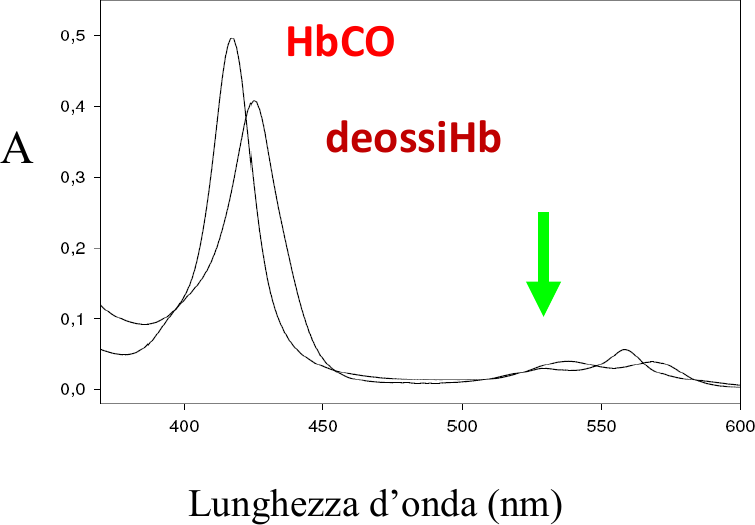
\includegraphics[width=0.6\textwidth]{abs_Mb_cropped.png}
    \caption{Spettri di assorbimento della CarbossiMb e della DeossiMb.}
\end{figure}
% [commento sul grafico]
Il grafico precedente mostra chiaramente questa differenza. Nonostante sia relativo all'emoglobina (Hb) rimane valido anche nel nostro caso dato che alla lunghezza d'onda di nostro interesse l'assorbimento è dovuto all'eme, che è il gruppo prostetico di entrambe le proteine.
Come si può osservare dal grafico, alla lunghezza d'onda di \qty{436}{\nano\meter} vi è un cambiamento drastico di assorbanza tra il caso in cui il CO (HbCO) è legato al Fe e quello in cui non lo è (deossiHb).

% [perché si misura la differenza di assorbanza e non l'assorbanza?]
La tensione misurata dall'oscilloscopio è l'unica misura dell'intensità di luce che attraversa il campione.
Per questa ragione conosciamo l'intensità del fascio a meno di un fattore moltiplicativo.
Questo però non ci impedisce di calcolare una misura relativa dell'assorbanza, cioè una differenza di assorbanza.
La differenza che calcoleremo sarà quella tra l'assorbanza ad un dato tempo $t$ e l'assorbanza del campione in assenza di perturbazioni (prima del flash).
Infatti

\begin{equation}
    \Delta A(t) = A(t) - A(t < t_0) = \log\left(\frac{I_0}{I(t)}\right) - \log\left(\frac{I_0}{I(t < t_0)}\right) =
    \log\left(\frac{I(t < t_0)}{I(t)}\right)
    \label{delta_abs}
\end{equation}

Dove $I_0$ rappresenta l'intensità della luce della lampada che incide sul campione e $t_0$ è l'istante in cui il flash laser arriva al campione.
Ovviamente noi non misuriamo direttamente $I(t)$ ma $\Delta V(t) = k I(t)$. Come è però chiaro da \eqref{delta_abs} questo fattore non fa alcuna differenza.

Come già anticipato, la cinetica di rilegame del CO alla Mb è composta dalla sovrapposizione di cinetiche più semplici che avvengono su scale di tempi diverse. Risulta di nostro interesse quello che avviene
anche su scale di tempi successive al flash inferiori ad \qty{1}{\micro\s}. L'oscilloscopio adoperato ci permette di arrivare senza difficoltà a frequenze di campionamento di $\qty{10}{\giga\sample \per \second}$.
A questa frequenza non siamo tuttavia in grado di registrare l'intera durata del fenomeno perché la memoria dell'oscilloscopio non è sufficiente a contenere una tale mole di dati. Inoltre a scale temporali grandi
non ci interessa avere una risoluzione temporale così alta.

Pertanto si è ripetuta la stessa misura impostando tre frequenze di campionamento diverse ma raccogliendo sempre circa \num{e5} campioni.
Le frequenze di campionamento sono state scelte in maniera da coprire rispettivamente \qty{1}{\micro\second}, \qty{100}{\micro\second} e \qty{10}{\milli\second}.

I tre segnali ottenuti sono stati combinati insieme rimuovendo le porzioni in cui si aveva sovrapposizione dei tempi.
Chiaramente il dato che si conserva è quello con frequenza di campionamento più alto. Le scale dei segnali ottenuti a frequenze diverse inoltre non sono esattamente identiche.
È stato necessario quindi riscalarli opportunamente. Poiché alla fine l'intero segnale verrà riscalato a sua volta, questo operazione è lecita.

Questa procedura è stata ripetuta con due campioni diversi.
Per entrambi si è ottenuta una concentrazione di \ce{CO} specifica portandoli all'equilibrio con delle miscele di azoto e \ce{CO}.
Nel primo caso la miscela aveva una pressione parziale di \ce{CO} pari a \qty{0.1}{\atm} mentre nel secondo di \qty{1}{\atm}.

\subsection{Riduzione del rumore}

I segnali registrati dall'oscilloscopio hanno inevitabilmente una componente di rumore. Si possono mettere in pratica alcune strategie per limitarne l'influenza sul segnale di nostro interesse.

La prima, e ovvia, cosa da fare è ripetere la misura più volte e fare una media. A tale scopo si può sfruttare una funzionalità dell'oscilloscopio che calcola direttamente la media su acquisizione multiple, ed evitando così di dover salvare più dati del necessario.
Sono state mediate $N=100$ acquisizioni, che significa che il rumore è stato attenuato di un fattore $1/\sqrt{N} = 10$.
La seconda consiste nel raccogliere una baseline, cioè il segnale misurato dall'oscilloscopio in assenza della luce della lampada. Il segnale così ottenuto viene poi sottratto al segnale regolare.
Questa pratica ovviamente non riduce il rumore termico ma è utile a rimuovere ogni tipo di interferenza che ha una certa periodicità.

% [drift PMT]
Per la scala di tempi più lunga, cioè \qty{10}{\milli\second}, è importante tenere in considerazione l'effetto di \emph{drift} del fotomoltiplicatore. Questo effetto provoca una decrescita nel tempo della tensione prodotta dal PMT a parità di intensità luminosa incidente.
Per eliminare questo effetto si registra una seconda baseline, questa volta nella condizione in cui la luce della lampada arriva al PMT.
La nuova baseline non viene semplicemente sottratta come nel caso precedente. Per prima cosa tutti i valori della baseline vengono divisi per il valore iniziale.
Si ottiene così una serie di dati che parte da 1 e gradualmente decresce. Dividendo poi il segnale per la baseline normalizzata si risale al segnale privo dell'effetto di drift.
Questa procedura aggiuntiva non è necessaria alle scale di tempi più brevi perché l'effetto del drift risulta trascurabile.

\section{Modello cinetico e analisi dei dati}

% [Modello cinetico del rilegame, geminato - bimolecolare]

Abbiamo già visto che il flash laser provoca la rottura del legame tra il \ce{Fe} e il \ce{CO}. Se l'energia cinetica del \ce{CO} è sufficiente, esso può fuoriuscire dalla proteina e andare in soluzione.
Altrimenti rimane all'interno della proteina ma sempre slegato dall'eme. Queste due fasi prendono il nome rispettivamente di fase bimolecolare e fase geminata.

Il modello che utilizziamo per descrivere la cinetica di rilegame contempla anche un quarto stato, detto stato trappola. In questo stato il \ce{CO} si trova ancora all'interno della proteina ma non è in grado
né andare in soluzione né di rilegarsi senza prima prima ritornare allo stato geminato. Di seguito è riportato un diagramma che illustra
tutti gli stati del modello cinetico utilizzato e tutte le transizioni permesse.

\begin{figure}[H]
    \centering
    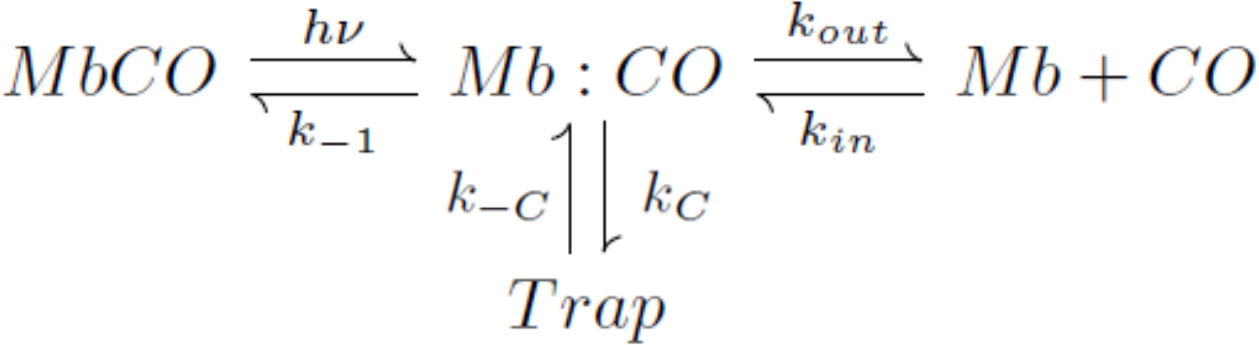
\includegraphics[width=0.6\textwidth]{kinetics_trimmed.png}
    \caption{Diagramma del modello cinetico.}
\end{figure}

Da questo schema è immediato dedurre il sistema di equazioni differenziali che descrive la cinetica.

\begin{equation}
    \begin{dcases}
        \frac{d}{dt} \ce{[Mb{:}CO]} = k_{-c} \ce{[Trap]} - (k_{-1} + k_c + k_{out}) \ce{[Mb{:}CO]} + k_{in} \ce{[Mb]}\ce{[CO]} \\
        \frac{d}{dt} \ce{[Mb]} = k_{out} \ce{[Mb{:}CO]} - k_{in} \ce{[Mb]}\ce{[CO]} \\
        \frac{d}{dt} \ce{[Trap]} = k_c \ce{[Mb{:}CO]} - k_{-c} \ce{[Trap]}
    \end{dcases}
    \label{kinetics_eqdiff}
\end{equation}

In queste equazioni ne manca una che descriva la variazione di \ce{[CO]}, ma non è necessaria dato che \ce{[Mb]} e \ce{[CO]} differiscono solo per una costante.
Infatti ogni volta che una molecola di \ce{CO} fuoriesce dalla proteina il numero di Mb senza CO e il quello di molecole di CO libere in soluzione aumentano di un'unità. La stessa cosa vale nel verso opposto.

% [noi misuriamo la differenza di conc. ma le equazioni rimangono le stesse]

Per la legge di Lambert-Beer, sappiamo che l'assorbanza del campione è proporzionale alla concentrazione di mioglobina.
Alla lunghezza d'onda a cui effettuiamo la misura di assorbimento, la variazione di assorbanza è dovuta unicamente alla formazione di deossiMb (cioè mioglobina con il CO slegato dall'eme). Inoltre, nella condizione di equilibrio,
tutta l'emoglobina presente in soluzione lega il CO. Siccome la differenza di assorbanza che misuriamo è fatta usando questa condizione come riferimento, quando la concertazione totale di deossiMb è nulla anche $\Delta A$ è nulla.
Pertanto è lecito scrivere

\[\Delta A(t) \propto \ce{[Mb{:}CO]} + \ce{[Mb]} + \ce{[Trap]} \]

Poiché la fotolisi ha un'efficienza del 100\%, l'assorbimento negli istanti successivi al flash è dovuto a tutte le proteine di Mb presenti in soluzione. Per questa ragione possiamo riscalare il nostro segnale
in modo che il suo massimo assoluto corrisponda alla concentrazione di mioglobina nel campione, ovvero \qty{17}{\micro\molar}.
In questo modo conosciamo l'andamento nel tempo della somma delle tre concentrazioni scritte sopra.

\subsection{Stima dei parametri ignoti}
% Vogliamo determinare tutte le variabili
Le informazioni di cui disponiamo a questo punto sono sufficienti per fare una stima delle costanti di velocità che compaiono nel sistema \eqref{kinetics_eqdiff} e delle concentrazioni iniziali.
Per fare ciò bisogna risolvere il sistema per via numerica e minimizzare, sempre numericamente, lo scarto quadratico tra la soluzione numerica del sistema e la misura.
Ad ogni step dell'iterazione dell'algoritmo di ottimizzazione è pertanto necessario risolvere il sistema con i nuovi parametri inferiti.
I valori iniziali utilizzati in questa procedura non sono scelti casualmente ma sono basati su un fit già eseguito in passato.

Questo metodo ci permette di eseguire un fit contemporaneamente per le due misure fatte a pressioni di \ce{CO} diverse.
Infatti è sufficiente minimizzare una funzione che sia la somma degli scarti quadratici dei due casi.
Naturalmente le concentrazioni iniziali differiscono, quindi tra i parametri per cui si esegue l'ottimizzazione è necessario includere
condizioni iniziali diverse del sistema \eqref{kinetics_eqdiff} e risolverlo separatamente per ciascuno dei due set di condizioni iniziali.

% [grafico fit]
\begin{figure}[H]
    \centering
    % 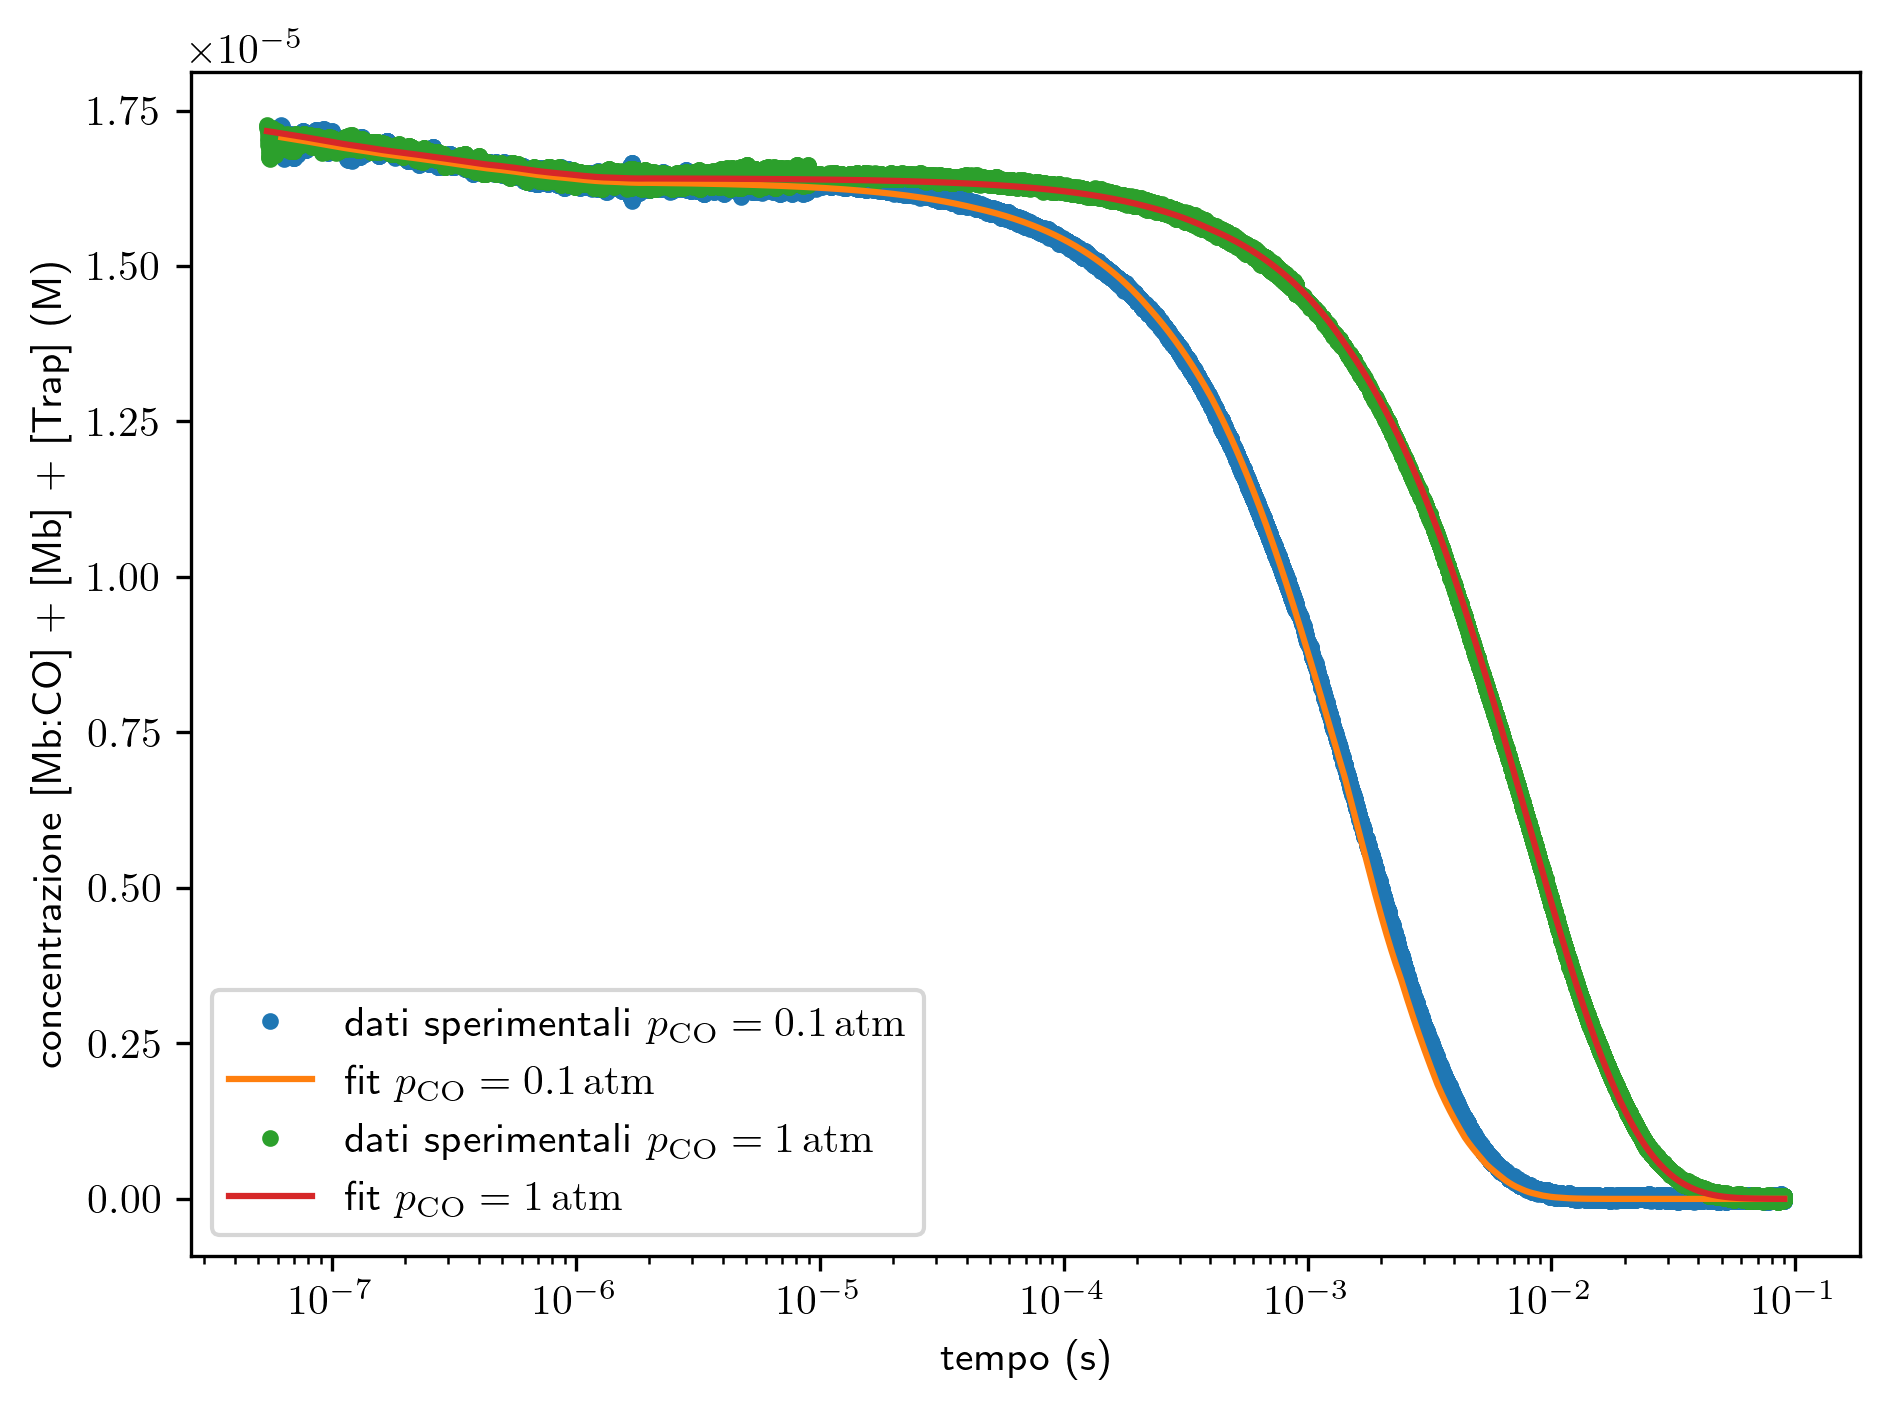
\includegraphics[width=0.6\textwidth]{fit2.png}
    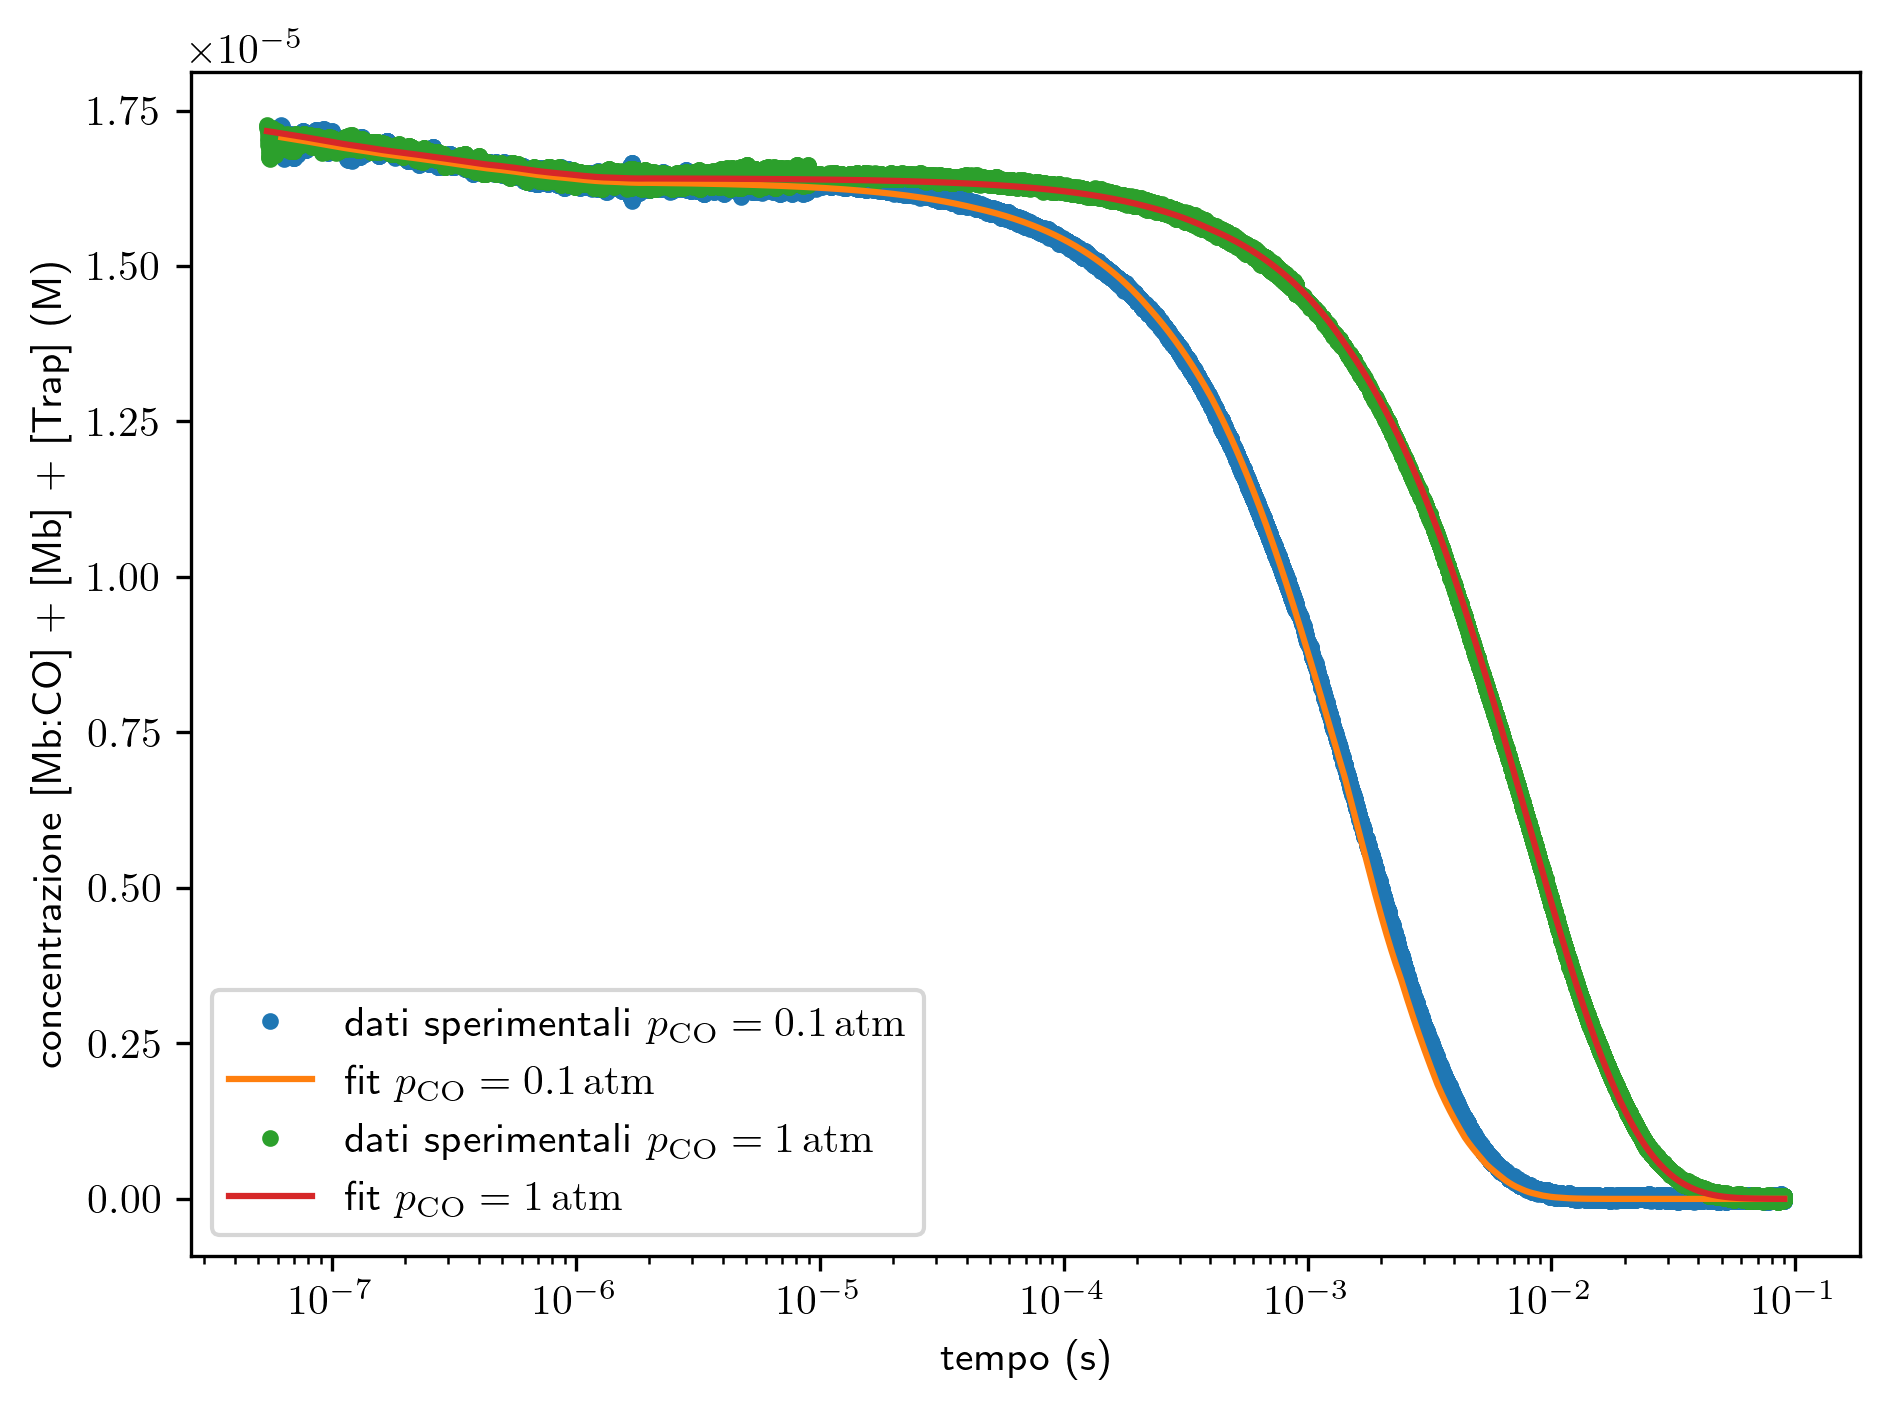
\includegraphics{fit2.png}
    \caption{TODO}
\end{figure}

\begin{table}[H]
    \begin{center}
        \footnotesize%
        \begin{tabular}{ccccc}
            \toprule
            $k_{-1}$ & $k_{out}$ & $k_{in}$ & $k_{c}$ & $k_{-c}$ \\
            (\unit{\s^{-1}}) & (\unit{\s^{-1}}) & (\unit{\molar^{-1}.\s^{-1}}) & (\unit{\s^{-1}}) & (\unit{\s^{-1}}) \\
            \midrule
            299999.68750000006 & 6499978.303914831 & 14999971.389751548 & 10000000.0 & 10000004.768372059 \\
            \bottomrule
        \end{tabular}
    \end{center}
    \caption{TODO}
\end{table}


\begin{table}[H]
    \begin{center}
        \footnotesize%
        \begin{tabular}{lcccc}
            \toprule
            $p_{\ce{CO}}$ & \ce{[Mb{:}CO]_0} & \ce{[Mb]_0} & \ce{[Trap]_0} & \ce{[CO]_0} \\
            (\unit{\atm}) & (\unit{\molar}) & (\unit{\molar}) & (\unit{\molar}) & (\unit{\molar}) \\
            \midrule
            1 & \num{1.71e-5} & 0 & 0 & \num{9.12e-4} \\
            0.1 & \num{1.71e-5} & 0 & 0 & \num{1.80e-4} \\
            \bottomrule
        \end{tabular}
    \end{center}
    \caption{TODO}
\end{table}
Dal grafico notiamo che a tempi inferiori a \qty{10}{\micro\s} la concentrazione di deossiMb è uguale in entrambi in casi.
A tempi più lunghi invece inizia a decadere a velocità diverse. La decrescita che si verifica per $ t < \qty{10}{\micro\s}$ infatti è
dovuta al rilegame della fase geminata. Questo processo è indipendente dalla concentrazione di \ce{CO} perché avviene all'interno della proteina,
quindi in un ambiente isolato dal solvente. Per tempi $ t > \qty{10}{\micro\s}$ si iniziano a vedere gli effetti del rilegame della fase bimolecolare.
In questa situazione è necessario che una molecola di \ce{CO} collida con una proteina di Mb affinché ritorni al suo interno.
Ciò significa che la velocità di questo processo dipende dalla probabilità che si verifichi un urto per unità di tempo. I due fattori che
influenzano principalmente questo dato sono la concentrazione di \ce[CO] e la temperatura.
In questi dati la temperatura del campione era mantenuta a \qty{20}{\celsius}, quindi la differenza che osserviamo è dovuta esclusivamente
alla diversa concentrazione di \ce{CO}.

\begin{figure}[H]
    \centering
    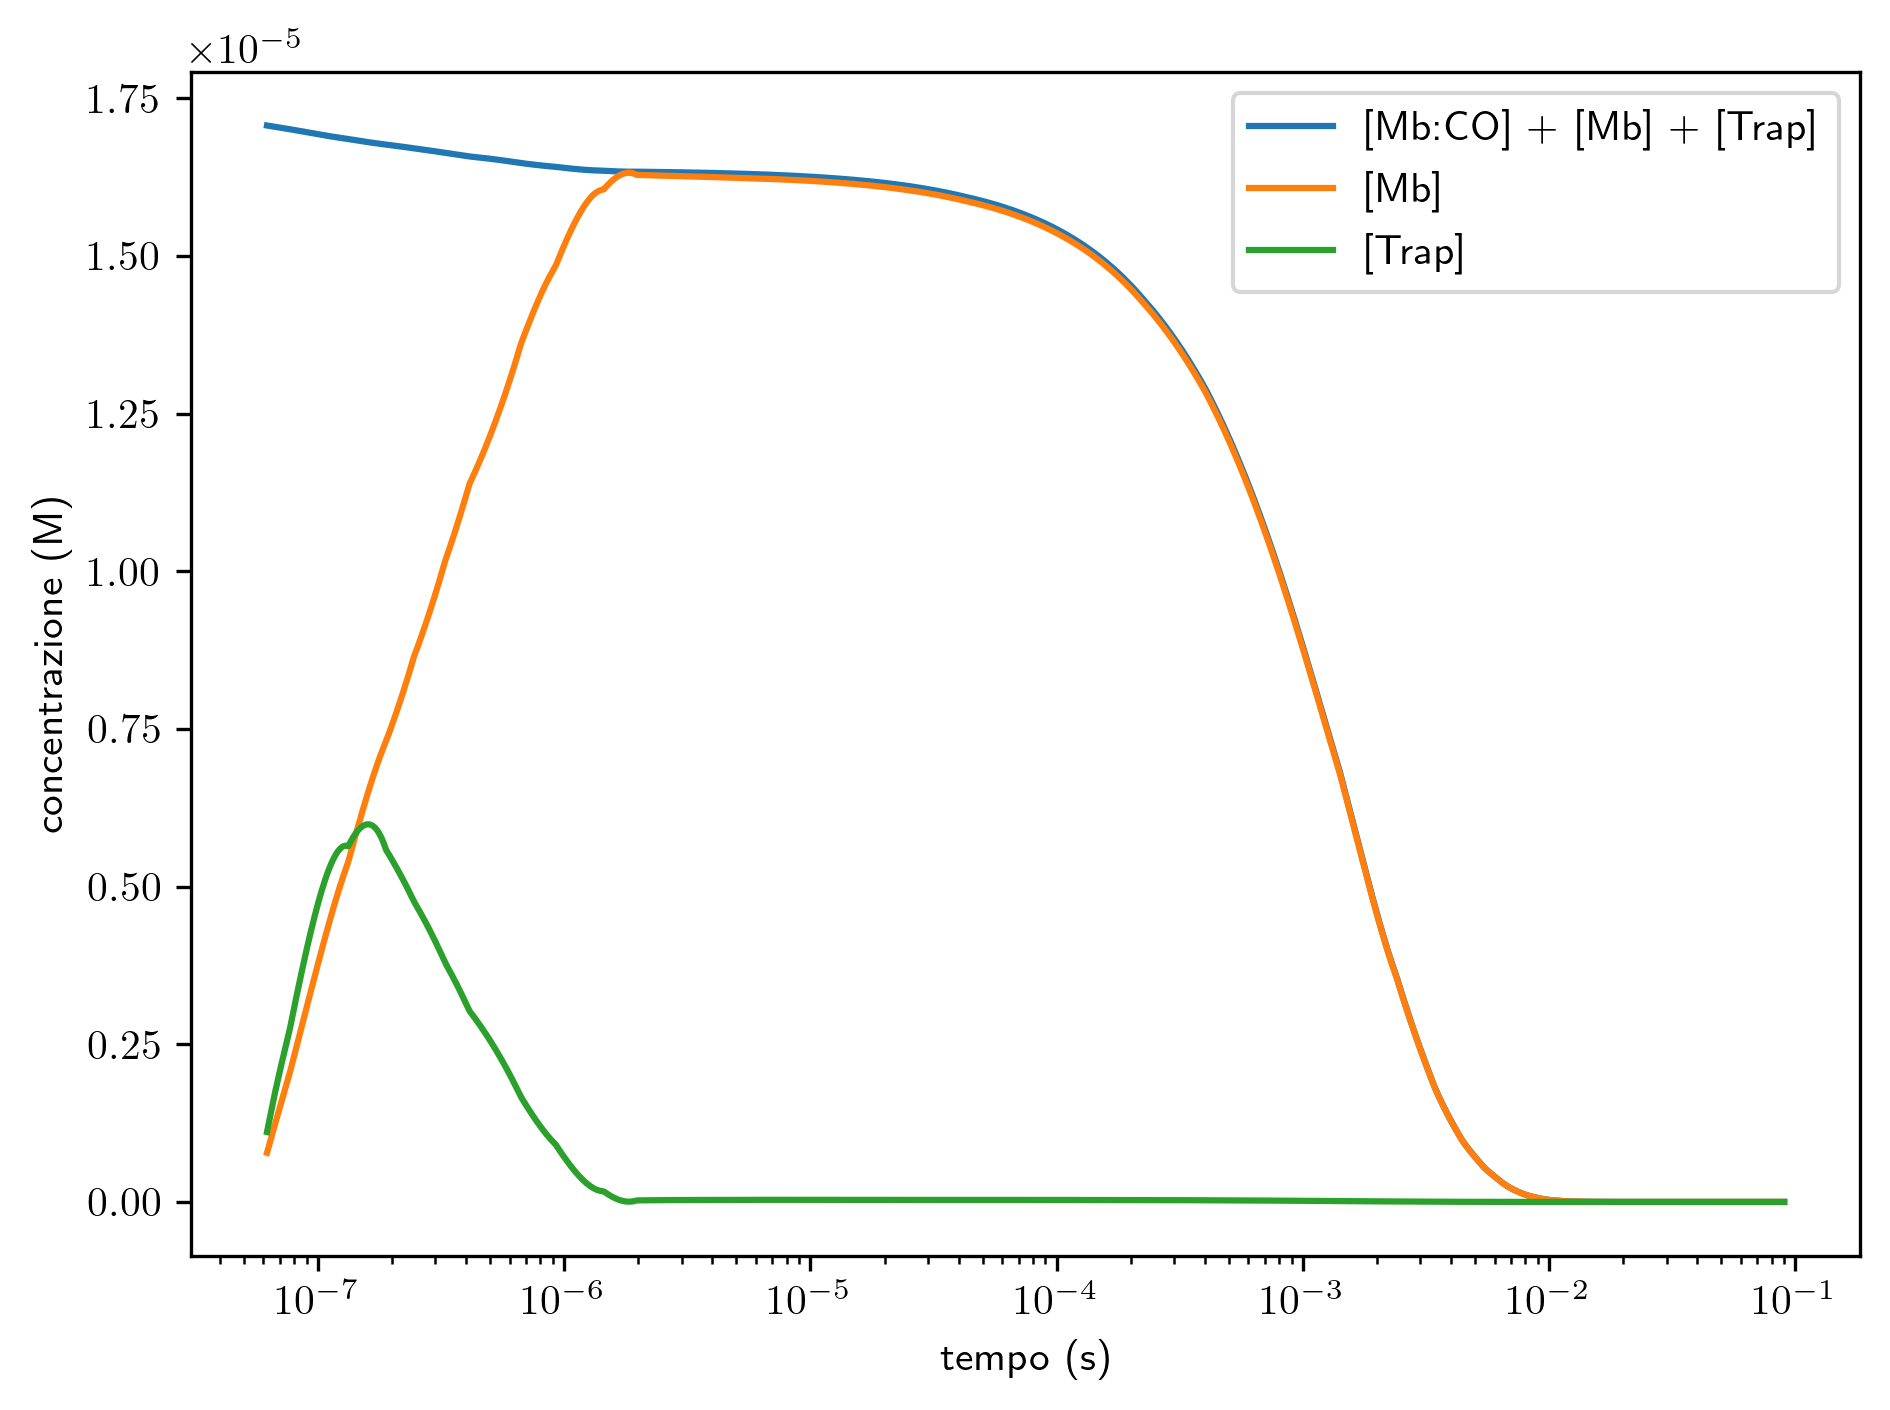
\includegraphics{tot_mb_trap.png}
    \caption{$p_{\ce{CO}} = \qty{1}{\atm}$}
\end{figure}

Questo secondo grafico da un più chiara visione di quello che avviene. Immediatamente dopo il flash quasi tutta la Mb si trova nello stato geminato.
Poi vediamo che una piccola parte del geminato si rilega (piccola decrescita della curva blu) mentre la larga maggioranza dei \ce{CO} esce in soluzione.
Questo è testimoniato dal rapido aumento della concentrazione \ce{[Mb]}. Nel giro di circa \qty{1}{\micro\second} il geminato scompare e la soluzione
è dominata dalla fase bimolecolare, cioè quella in cui Mb e CO sono separati.

\end{document}
